\documentclass[]{article}

\usepackage{graphicx}
\usepackage{amssymb}
\usepackage{color}
\usepackage{hyperref}
\usepackage{float}

\bibliographystyle{abbrv}

\begin{document}
    \title{The Ergo Platform}
    \author{Dmitry Meshkov}

    \date{January 25, 2019\\v1.0}

    \maketitle

    \begin{abstract}
        This document contains the general idea of Ergo platform and a high-level overview of its main
        features. More details can be found in dedicated papers cited.
    \end{abstract}

    \section{Vision}

    Ergo platform development began in 2017 after several years of research and prototype
    implementations. Despite the huge hype around cryptocurrencies, the technology itself has
    been stuck close to its initial stage. In pursuit of high profits and popularity, developers claimed
    implementations of blockchain 2.0, 3.0 and so on, mostly in opposition to the main advantage of
    cryptocurrencies --- decentralization --- and teams have simply promised that decentralization will
    be achieved at some point in the future.

    In contrast, the idea of Ergo platform is to implement ready-to-use ideas keeping the network
    truly decentralized. It may be called a ``blockchain 1.1'' implementation --- a major update to
    blockchain technology instead of revolutionary breaking changes. The objective of Ergo is to be
    the platform that is truly useful for blockchain-demanding decentralized applications, and to be
    survivable in the long-term thus enabling it to be a powerful store of value. Technical and economic
    solutions that will allow it to achieve this are summarized in the following sections.

    \section{Consensus}

    Consensus protocol of Ergo --- Autolykos --- is based on the well-known
    Proof-of-Work (``PoW'')
    consensus algorithm. PoW was chosen for several reasons including that PoW protocols are widely
    studied, have high security guarantees, and are friendly to light clients.

    However, existing PoW protocols have known drawbacks: ASIC-equipped miners produce
    blocks orders of magnitude faster than CPU or GPU-equipped miners, moreover, they unite in
    mining pools and just a few pool operators control the network as a result, sometimes in a non-transparent
    manner. This potentially represents a single point of failure for a network and poses
    a severe threat to long-term survivability.

    The general method to reduce the advantage of ASICs is to use memory-hard computations.
    Autolykos is based on the k-sum problem, that is similar to a known memory-hard Equihash
    PoW~\cite{biryukov2017equihash}. In addition, Autolykos is a variant of a Schnorr signature and thus mining is not
    possible without access to the private key making the underlying puzzle non-outsourceable.

    These two properties of Ergo platform prevent the centralization of the network around pool
    operators and ASIC manufacturers, and return Ergo back to the original one-CPU-one-vote idea
    from the Bitcoin whitepaper~\cite{nakamoto2008bitcoin}.

    \section{Clients}

    It is almost impossible to use existing cryptocurrencies without the help of trusted third-parties.
    To receive even a small amount of coins in a trustless fashion, a client must download and process
    gigabytes of data to synchronize with the network, which may take several weeks even on highend
    hardware, not to mention mobile devices. It is therefore no surprise that most users prefer
    to use trusted solutions for wallets, exchanges, block explorers and so on.

    Ergo was designed to be maximally user-friendly in the sense of decentralization. One of
    important properties of PoW is that it enables verification of the work done without downloading
    the full chain. Ergo block headers support NiPoPoW~\cite{kiayias2017non} proofs, allowing light clients to
    synchronize with the network by downloading less than a megabyte of data. In addition, Ergo uses
    authenticated state~\cite{reyzin2017improving} and for any transaction included, a client may download a proof of its
    correctness. Thus, regardless of the blockchain size, a regular user with a smart-phone can join
    the network and start using Ergo with the same security guarantees as a full node.

    \section{Survivability}

    If Ergo or any other cryptocurrency is to be a store-of-value, long-term survivability and the
    confidence of users in the platform’s long-term survivability is essential.

    To survive in the long-term, Ergo prefers well-tested solutions. If there isn't already a well-tested
    solution for some problem, we perform our own research and the number of peer-reviewed
    papers from the Ergo development team is already extensive:~\cite{reyzin2017improving,meshkov2017short,chepurnoy2018systematic,chepurnoy2018self,chepurnoy2018checking,duong2018multi}

    To be survivable, the network should adopt to changing environment without the intervention
    of trusted parties (such as a ``core developer'' team). Ergo's on-chain miner voting protocol
    allows gradual changes in a large number of parameters including:

    \begin{itemize}
        \item Maximum block size
        \item Maximum cumulative computational cost of a block
        \item Computational cost of contracts
        \item Storage fee factor (see Section~\ref{sec:economy} for details)
    \end{itemize}

    For more fundamental changes Ergo is going to follow a soft-forkability
    approach --- if an
    overwhelming majority of the network accepts a new feature, it is activated, however, old nodes
    who do not upgrade continue to operate normally and just skip over this feature validation.

    \section{Economy}
    \label{sec:economy}

    To achieve survivability, Ergo provides economic improvements in addition to the technical
    ones, most central of which is a storage fee component which plays an important role for Ergo`s
    stability: if an output remains in state for 4 years without being moved, a miner may charge
    small fee for every byte kept in the state. If value of the output is less than a required fee to
    pay, then the output will be removed from the state.

    Thus, storage fee component is similar to regular cloud storage services, however, it is new for
    cryptocurrencies and has several important consequences. First, Ergo mining will always be
    stable, unlike Bitcoin and other PoW currencies, in which mining may become unstable after the
    initial emission~\cite{carlsten2016instability}. Second, state size growth becomes controllable and predictable,
    reducing hardware requirements for Ergo miners. Third, by collecting a storage fee from outdated boxes,
    miners return coins to circulation, preventing steady decrease of circulating supply due to lost
    keys~\cite{wsj2018}.

    Finally, it allows emission to be stopped quite soon. Ergo emission will
    last for 8 years --- for the
    first 2 years 75 Erg (Erg is Platform's native coin) will be issued per block with a 2 minute block
    interval and after that the block reward will be reduced by 3 coins every 3 months (see Fig.~\ref{fig:emission}).
    To fund the Ergo development, during the first 2.5 years, the part of the block reward that
    exceeds 67.5 will go to a treasury instead of a miner. Ergo emission will start from zero with no
    pre-mine. As proof-of-no-pre-mine we are going to use news headlines, like Satoshi, as well as
    latest block ids from Bitcoin and Ethereum.

    \begin{figure}[H]
        \centering
        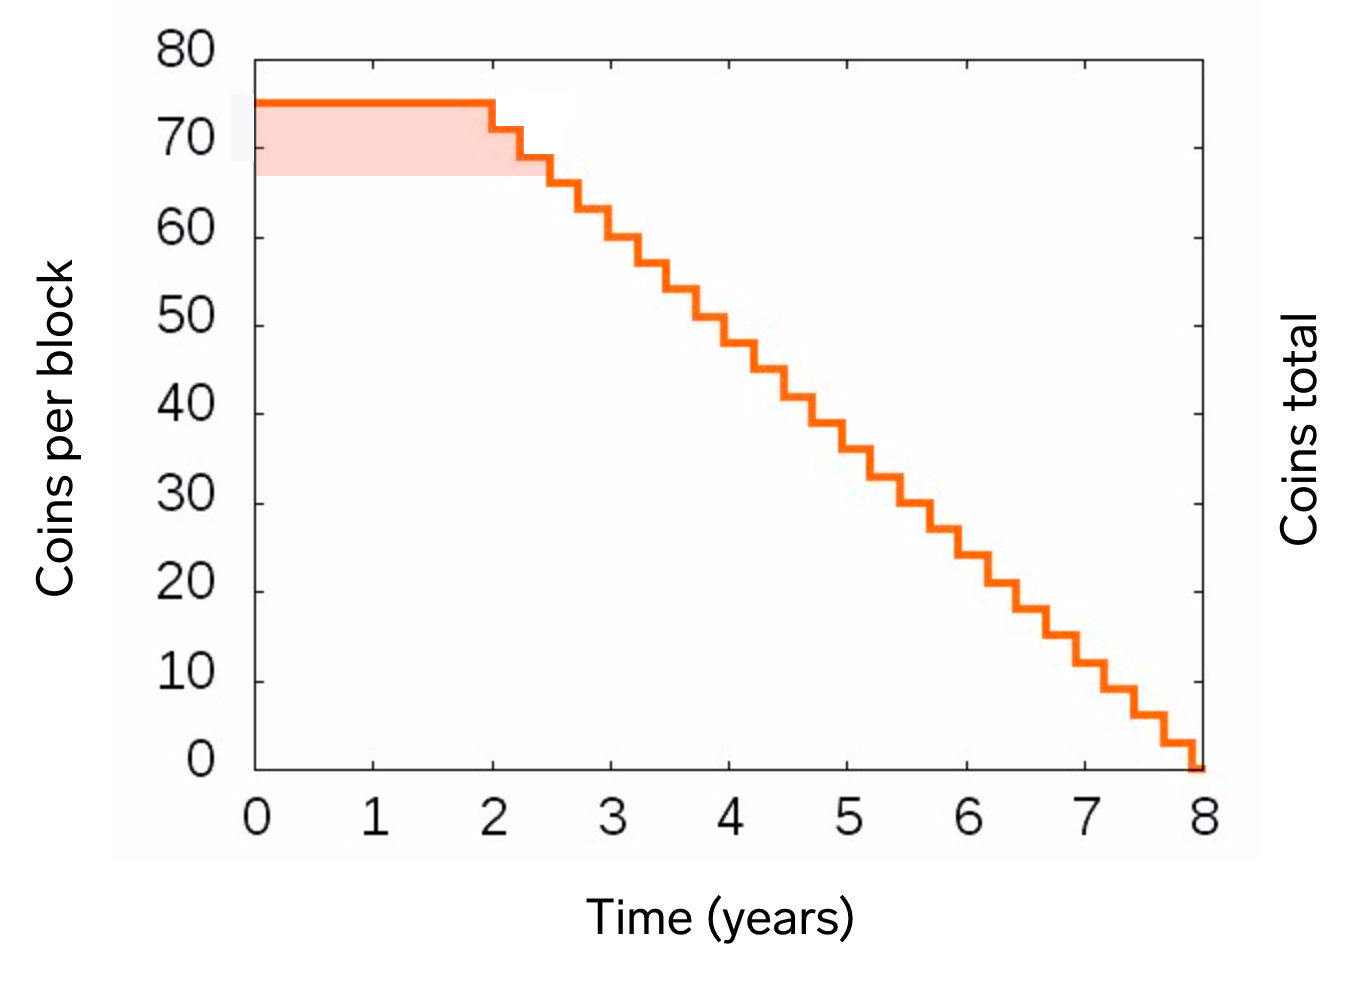
\includegraphics[width=\textwidth]{emission.jpg}
        \caption{Ergo emission curve
        \label{fig:emission} }
    \end{figure}


    \section{Applicability}

    To survive, a blockchain must have a user base. DApps and offchain protocols may be
    implemented in a truly decentralized way due to light clients, however, they also require a useful
    and safe smart contract language. Ergo smart contracts are based on a Bitcoin-like UTXO
    model, where every output is protected by some script. If the scripting language is rich enough,
    it enables writing of Turing-complete contracts~\cite{chepurnoy2018self} while avoiding ad-hoc solutions for
    program halting like gas in Ethereum. While having significantly more versatility than Bitcoin
    script, Ergo script only contains operations, that allow estimation of script complexity before
    execution, which prevents various DoS attacks. However this instructions set is enough to
    easily write any possible program --- ErgoScript was proven to be Turing complete~\cite{chepurnoy2018self}. The
    cryptographic part of Ergo script is based on sigma protocols and naturally supports threshold
    m-of-n signatures, ring signatures and more.

    \section{Community}

    In relation to community building, for now, we have followed an approach of focusing nearly
    exclusively on research, development, analytics and testing while letting the community build
    organically at a slow pace. We believe this has allowed us to attract a small but quality following
    of early enthusiasts who share a similar philosophy, while allowing the development team to
    focus on its many tasks. However, as we approach the completion of Ergo's final testnet and the
    launch of mainnet, our community building efforts will intensify substantially and this important
    aspect of a successful platform launch will not be overlooked.

    \section{Conclusions}

    In this brief high level summary of Ergo Platform, we hope that we have highlighted the most
    distinguishing characteristics of this new platform as well as the philosophy of the Ergo Platform
    development team and why this platform may be of keen interest to a diverse base of users,
    miners, traders and long-term investors in cryptocurrency.

    \bibliography{references}

\end{document}
